\section{Michelson-Interferometer}
\subsection{Versuchsbeschreibung}

Bei diesem Versuchsteil soll die Stabilität des Versuchsaufbaus, die Auswirkung äußerer Einflüsse sowie die Kohärenzlänge des verwendeten Lasers untersucht werden. Da uns ein neuer Versuchstisch zur Verfügung gestellt wurde, sollte auch ein Vergleich mit dem bisherigen durchgeführt werden.


\begin{figure}[H]
 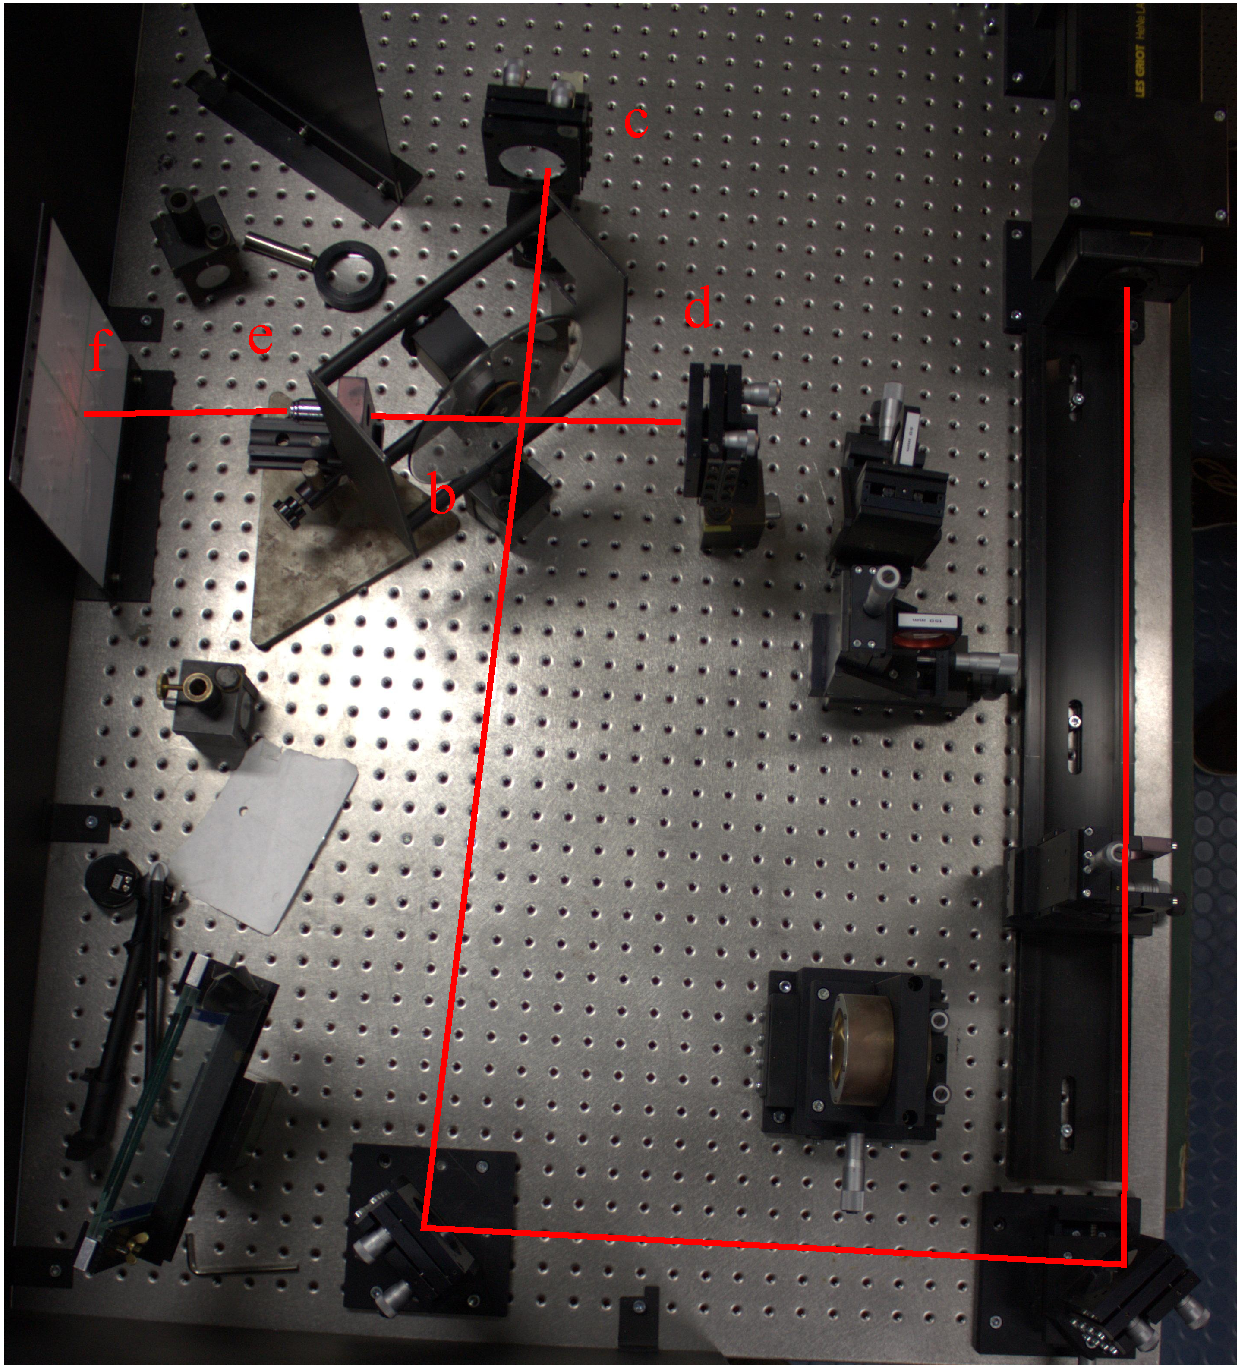
\includegraphics[width=\textwidth]{BilderAufbau/Michelson.pdf}
 \caption{Draufsicht auf das Interferometer}
 \label{aufbau_interferometer}
\end{figure}

Der Aufbau (Abb. \ref{aufbau_interferometer}) besteht aus dem Laser (a) und einem Michelson-Interferometer. Bei diesem wird am Strahlteiler (b) der Laserstrahl in zwei Komponenten geteilt. Ein Teil geht in Einfallrichtung gerade weiter und trifft auf den Spiegel (c), wo er reflektiert wird. Nachdem er zusätzlich am Strahlteiler reflektiert wurde, trifft er auf den Schirm. Der andere Teil wird bereits beim ersten Auftreffen auf den Strahlteiler reflektiert und gelangt über einen weitere Spiegel (d) ebenfalls auf den Schirm (f). Das dort beobachtete Interferenzmuster kann zusätzlich mit einem Mikroskopobjektiv (e) vergrößert werden.  

Ist der Versuchsaufbau stabil aufgebaut und sind die äußeren Störungen nicht zu groß, so sollten die Weglängen der beiden Strahlen auf dem Schirm nur orts- nicht jedoch zeitabhängig sein. Die zeitliche Stabilität des Interferenzmusters dient uns somit als Mass für die Qualität und Empfindlichkeit des Aufbaus.

Ist ein stabiles Interferenzmuster eingestellt, so kann die Kohärenzlänge des Lasers bestimmt werden. Dazu wird einer der beiden Spiegel (bei uns c) so lange verschoben bis das Interferenzmuster zusammenbricht. Der Weglängenunterschied zwischen b-d-b und b-c-b bei dem gerade noch Interferenz erkennbar ist, entspricht der Kohärenzlänge.


\subsection{Durchführung und Auswertung}

Wir haben das Michelson-Interferometer zuerst mit dem alten Tisch analog wie in Abb \ref{aufbau_interferometer} aufgebaut. Dabei konnten wir allerdings kein wirklich stabiles Interferenzmuster erreichen. Bei Vermeidung sämtlicher Störungen (Luft anhalten etc.) war zwar regelmäßig für kurze Zeit ein Muster zu sehen, es verschwand aber innerhalb von weniger als einer Sekunde wieder. Für die benötigten Belichtungszeiten von einigen Minuten ist dieser Versuchsaufbau also ungeeignet.
Daher haben wir anschließend den neuen Versuchstisch untersucht. Dieser hat vier luftgefüllte Dämpfer, welche eine wesentlich bessere Entkopplung von der Umgebung versprechen. Wir haben hier also das Interferometer erneut aufgebaut (Abb \ref{aufbau_interferometer}). Das Interferenzbild (Abb. \ref{michelson_interferenzmuster}) ließ sich hier stabil einstellen und auch sehr gut photografieren. Innerhalb von Belichtungszeiten bis zu 30s veränderte es sich nicht und ergab ein scharfes Bild, längere Zeiten erlaubte leider die verwendete Kamera nicht. Ein Antippen des Tisches führte zu einem kurzfristigen Verschwinden des Interferenzmusters, es tauchte nach ca. 5-10 s wieder auf.  Reden führte zu einem leichten Flackern des Bildes, ohne es jedoch verschwinden zu lassen. Erhitzen der Luft führte zu einem Wandern des Musters, also zu einem Drift der Weglänge.

Zur Bestimmung der Kohärenzlänge des NeHe-Lasers haben wir dann den Spiegel (c) verschoben. Um größere Weglängendifferenzen zu erreichen haben wir dann auch das komplette Interferometer noch weiter nach "`vorne"' versetzt, als dies in Abb \ref{aufbau_interferometer} sichtbar ist. Trotzdem konnten wir kein Verschwinden des Interferenzmusters erreichen, da der Tisch uns Grenzen setzte. Der maximale Weglängenunterschied den wir einstellen konnten war:
\begin{align*}
 \Delta l & = 2 \cdot \overline{bc} - 2 \cdot \overline{bd} \\
          & = 2 \cdot (74 \pm 1) cm - 2 \cdot ( 6,5 \pm 0,5 ) cm \\
	  & = (135,0 \pm 0,2) cm
\end{align*}

Die Kohärenzlänge des Lasers sollte uns in diesem Versuch also keine Probleme bereiten. 

 
\begin{figure}[H]
 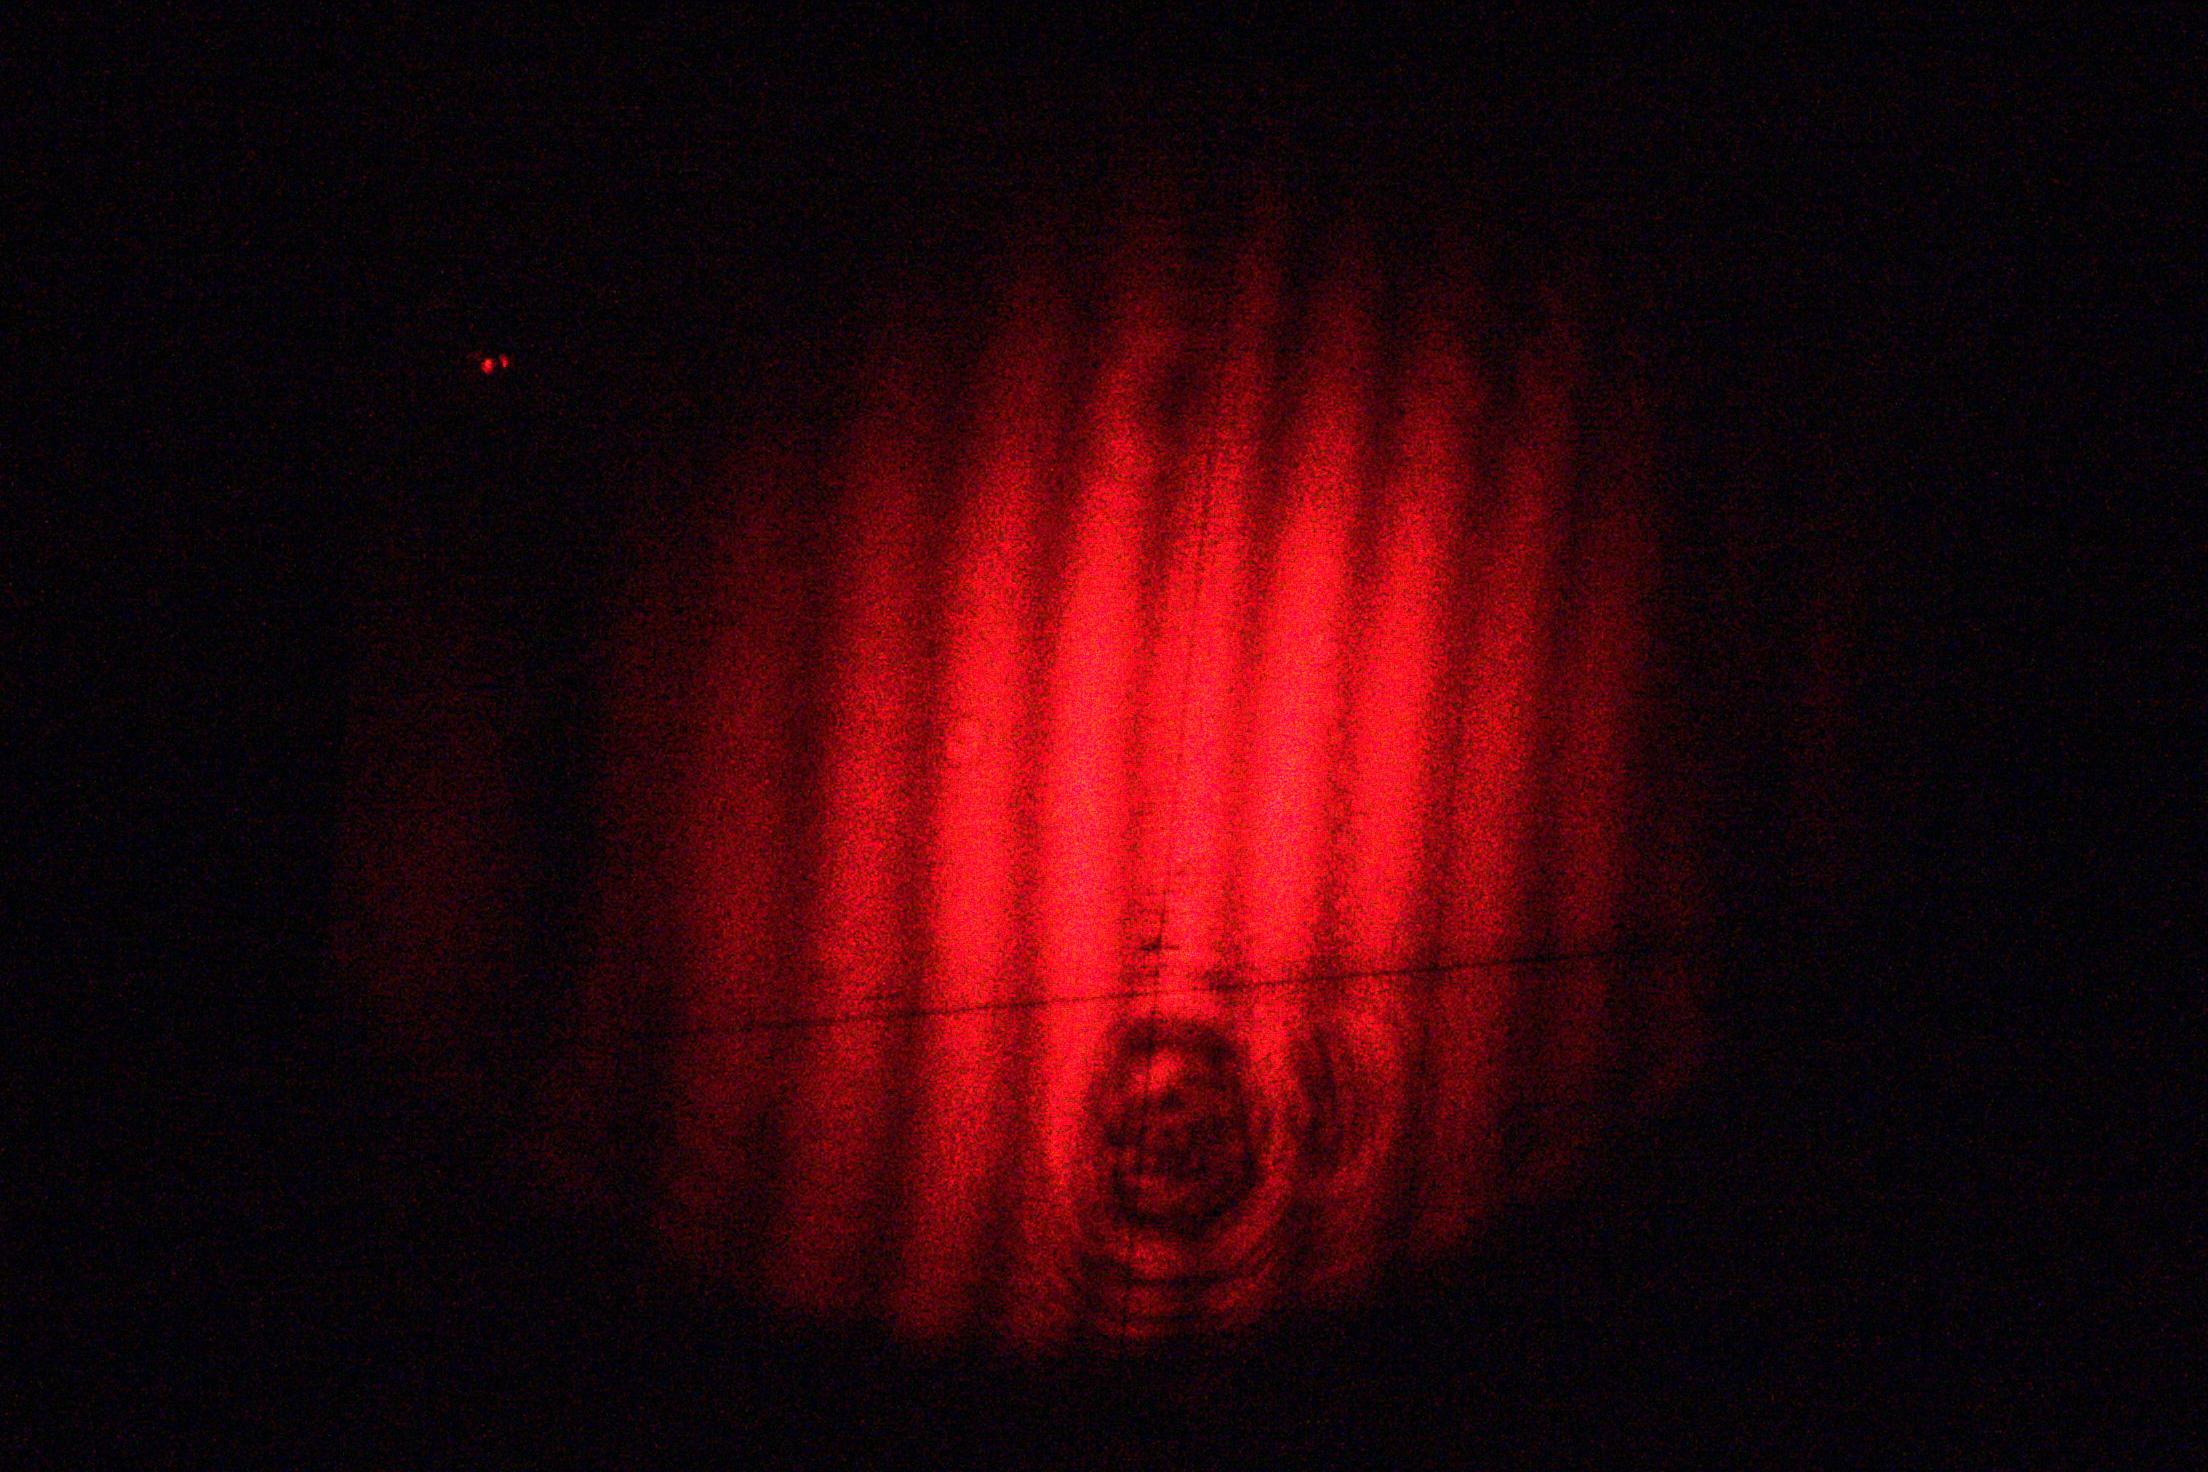
\includegraphics[width=\textwidth]{Photos/IMG_3881.jpg}
 \caption{Interferenzmuster}
 \label{michelson_interferenzmuster}
\end{figure}


\begin{figure}[H]
 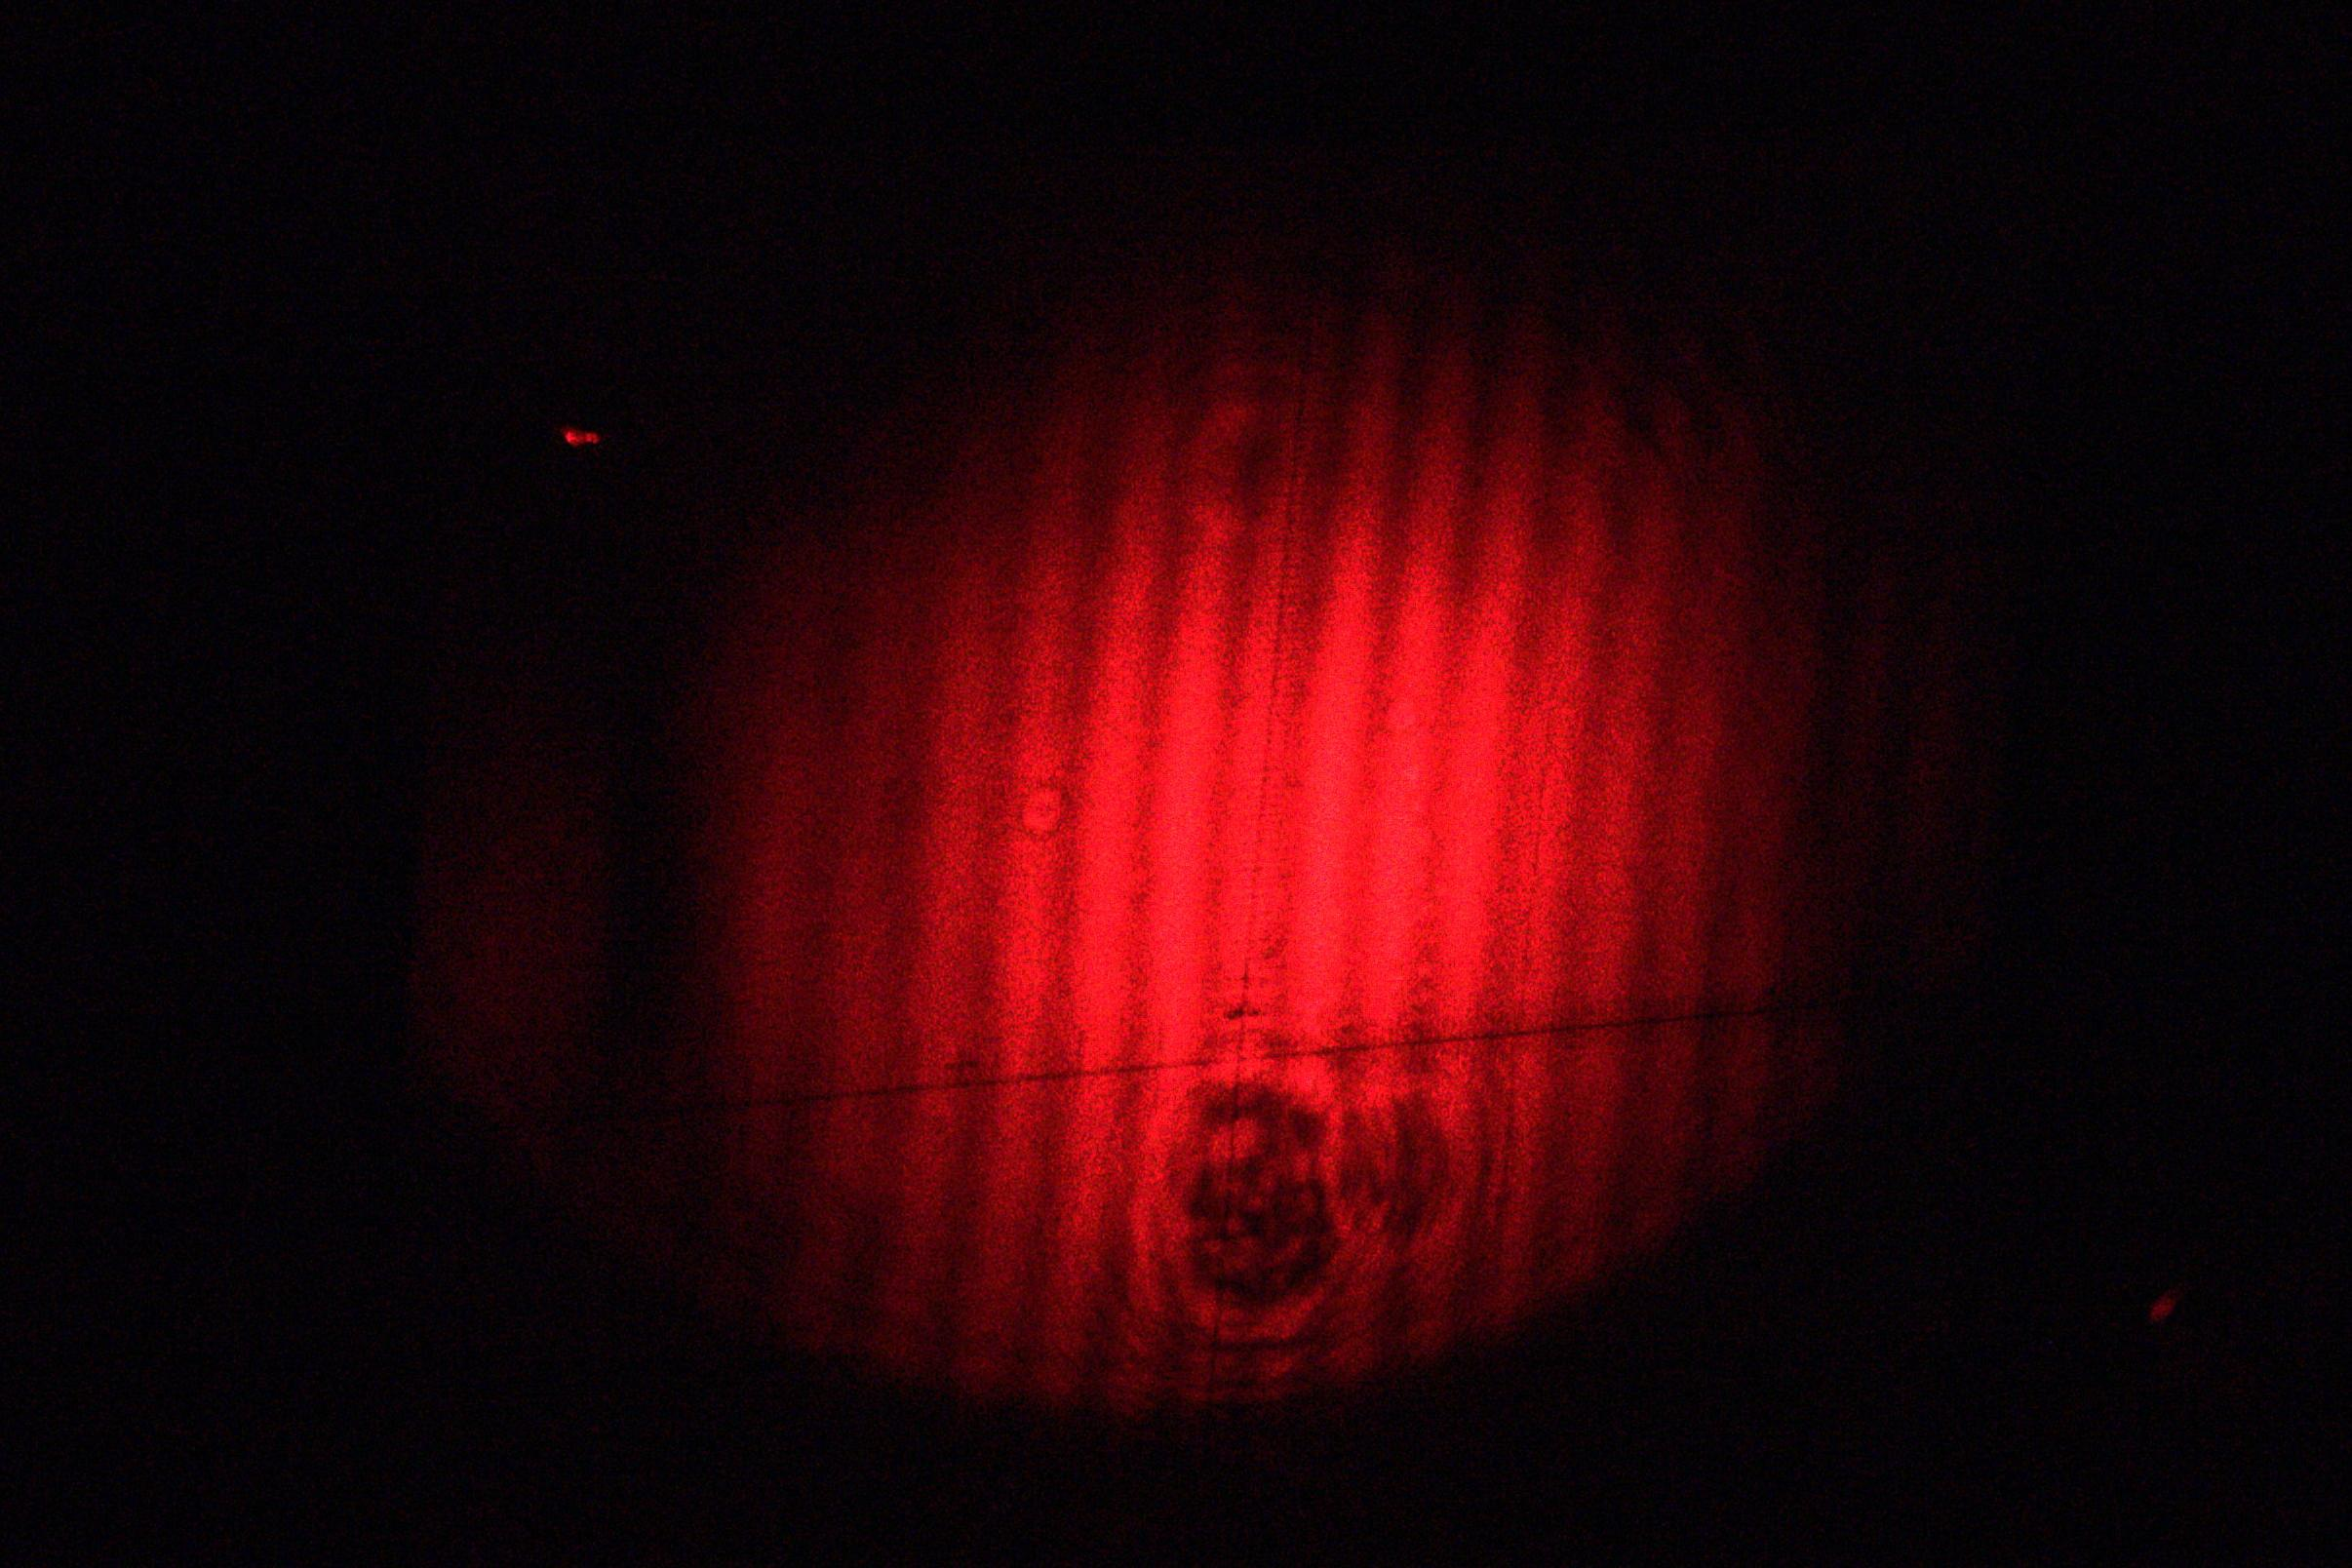
\includegraphics[width=\textwidth]{Photos/IMG_3887.jpg}
 \caption{Interferenzmuster}
\end{figure}